\documentclass{article}

\usepackage{neurips_2026}

\usepackage[utf8]{inputenc}
\usepackage[T1]{fontenc}
\usepackage{hyperref}
\usepackage{url}
\usepackage{booktabs}
\usepackage{amsfonts}
\usepackage{amsmath}
\usepackage{amssymb}
\usepackage{nicefrac}
\usepackage{microtype}
\usepackage{xcolor}
\usepackage{graphicx}

\graphicspath{{figures/}}

\newcommand{\E}{\mathbb{E}}
\newcommand{\F}{\mathcal{F}}
\newcommand{\norm}[1]{\left\lVert #1 \right\rVert}

\title{Replication and Predictable-Drift Diagnostics for FTS-Diffusion}

\author{%
  Anonymous Author(s)\\
  Anonymous Institution\\
  \texttt{anonymous@example.com}
}

\begin{document}

\maketitle

\begin{abstract}
Financial time-series generators are often evaluated by marginal stylized facts and downstream forecasting gains, but those criteria can miss protocol artifacts and artificial conditional mean predictability. We study FTS-Diffusion, an ICLR 2024 model based on scale-invariant subsequence clustering, pattern-conditioned diffusion, and learned pattern evolution. Our replication finds that S\&P 500 Train-on-Augmentation-Test-on-Real (TATR) conclusions depend strongly on the synthetic rollout: a six-seed continuous-rollout protocol reaches a mean best improvement of $84.9\%$, whereas independent 252-day blocks never improve over baseline and finish $193.2\%$ worse. We also fail to reproduce the Appendix B.3 SISC toy targets, with best average per-unit DTW $0.0321$ versus $0.01$ and best interval IoU $0.6418$ versus $0.784$. As an extension, we implement a fixed predictable-drift diagnostic. On real S\&P 500, GOOG, and ZC=F holdouts, the statistic lies inside asset-specific block-shuffle null bands. In a 100-seed hidden-drift experiment, the same statistic tracks exploitable artificial alpha: at sign persistence $p=0.85$, mean out-of-sample Sharpe is $7.68$ versus $0.08$ for an iid-sign control. The main lesson is that realistic-looking financial paths are not enough: synthetic finance benchmarks need protocol-explicit generation and direct checks for artificial alpha.
\end{abstract}

\section{Introduction}

Deep generative models are attractive for finance because historical market data are scarce, noisy, nonstationary, and not experimentally reproducible. Financial returns also exhibit heavy tails, weak raw-return autocorrelation, volatility clustering, and recurring shapes at irregular time scales \citep{cont2001stylized}. FTS-Diffusion \citep{huang2024fts} addresses the last property directly by discovering variable-length motifs and generating new trajectories motif by motif.

This paper is a replication and diagnostic-extension study. We do not introduce a replacement generator. Instead, we test whether the published downstream gains are robust to rollout details, whether the SISC toy-data targets are reproducible, and whether a simple predictable-drift statistic catches artificial alpha that marginal stylized facts may miss. The answer is mixed: the architecture is well motivated, but the downstream evidence is fragile because continuous Markov-chain rollouts and independent yearly blocks answer different questions.

We therefore extend the evaluation with a predictable-drift diagnostic. Under a fixed information vector
\begin{equation}
  \omega_t = (1, r_t, r_{t-1}, |r_t|, |r_{t-1}|)^\top,
\end{equation}
we measure whether the next return $r_{t+1}$ has a nonzero linear conditional mean under a bounded test class. This is not a proof of market efficiency or absence of arbitrage. It is a finite, reproducible check for an important failure mode: a synthetic generator can match tails and volatility clustering while introducing a simple, exploitable conditional drift.

\paragraph{Contributions.}
We make four contributions: a replication summary on S\&P 500, GOOG, and corn futures (ZC=F); a six-seed isolation of TATR rollout sensitivity; a documented Appendix B.3 SISC replication gap; and a predictable-drift diagnostic calibrated on real assets and validated by a 100-seed predictive-alpha experiment.

\section{Background: FTS-Diffusion}

FTS-Diffusion decomposes financial time-series generation into three modules \citep{huang2024fts}. Scale-invariant subsequence clustering (SISC) segments a univariate series into variable-length motifs using dynamic time warping (DTW) \citep{sakoe1978dtw} and DTW barycenter-style centroid updates \citep{petitjean2011dba}. Each segment is summarized by a pattern identity $p_m$, a duration scale $\alpha_m$, and a magnitude scale $\beta_m$. A pattern-conditioned diffusion model then generates concrete segments from motif conditions using a DDPM-style denoising objective \citep{ho2020ddpm}.

The long-horizon behavior is controlled by the pattern-evolution module, which learns
\begin{equation}
  (p_m,\alpha_m,\beta_m) \mapsto (p_{m+1},\alpha_{m+1},\beta_{m+1}),
\end{equation}
with a classification loss for the next pattern and regression losses for the next duration and magnitude scales. This separation is useful, but it also creates a sensitive interface: downstream results depend on how the learned state chain is initialized, reset, and sliced into synthetic training blocks.

\section{Replication protocol}

\paragraph{Assets and splits.}
The main datasets are daily Yahoo Finance close-price histories for S\&P 500, GOOG, and ZC=F. The S\&P 500 setup spans 1980--2020 and yields 10,088 trading days and 2,282 post-SISC segments with $K=14$. GOOG spans 2004--2020 with 3,776 trading days and 733 post-SISC segments with $K=11$. ZC=F spans 2000--2020 with 4,764 trading days and 629 post-SISC segments with $K=11$. We follow a chronological train/test design: the generator is fit on the training slice, and downstream predictors are evaluated on held-out real data.

\paragraph{Downstream benchmark.}
The main downstream benchmark is TATR: Train on Augmentation, Test on Real. The held-out real slice is divided into an initialization portion and a final real test portion. A one-day-ahead LSTM forecaster is trained on the real initialization portion plus $Y$ synthetic trading years, where one synthetic year has 252 days and $Y$ is swept across a fixed grid. The score is mean absolute percentage error (MAPE) on the final real test portion. We use paper-like LSTM settings: one-day ahead, window size 64, hidden size 32, two layers, MAE training loss, Adam with learning rate $10^{-2}$, and 100 epochs for the primary S\&P 500 runs.

\paragraph{Synthetic rollout variants.}
We compare three ways to produce the synthetic augmentation path.

\begin{itemize}
  \item \textbf{Independent fixed blocks:} generate independent 252-day blocks from the same fixed initial state.
  \item \textbf{Continuous chunked:} generate one continuous trajectory with the pattern-evolution chain, then split it into 252-day chunks for downstream training.
  \item \textbf{Continuous with scaler refit:} generate a continuous trajectory and refit the downstream scaler on the augmented training series.
\end{itemize}

These protocols use the same broad data budget but different Markov-chain connectivity. The distinction matters because the pattern-evolution module is the only component that carries long-horizon state across generated motifs.

\section{Replication results}

\subsection{TATR depends on the synthetic-series protocol}

Table~\ref{tab:tatr-summary} summarizes the six-seed S\&P 500 long-batch TATR result. Continuous protocols reproduce strong paper-like reductions in downstream MAPE, but independent fixed blocks do not. The contrast is also visible in Figure~\ref{fig:tatr-protocol}: continuous trajectories eventually cross below the real-only baseline, while independent blocks worsen as augmentation increases.

\begin{table}[h]
  \caption{Six-seed S\&P 500 TATR summary. Percentages are relative to each protocol's no-augmentation baseline; lower MAPE is better. Continuous trajectory protocols reproduce large best improvements, whereas the independent-block rollout never improves over baseline and finishes much worse.}
  \label{tab:tatr-summary}
  \centering
  \begin{tabular}{lrrlr}
    \toprule
    Protocol & Seeds & Baseline MAPE & Best change & Final change \\
    \midrule
    Continuous chunked, 1-day & 6 & 0.0589 & $-84.9\%$ & $-65.2\%$ \\
    Continuous + scaler refit, 1-day & 6 & 0.0630 & $-85.4\%$ & $-68.2\%$ \\
    Independent fixed blocks, 1-day & 6 & 0.0646 & $0.0\%$ & $+193.2\%$ \\
    Continuous chunked, 5-day & 6 & 0.0810 & $-85.2\%$ & $-77.5\%$ \\
    \bottomrule
  \end{tabular}
\end{table}

\begin{figure}[t]
  \centering
  
\includegraphics[width=0.92\linewidth]{02_tatr_protocol_contrast.pdf}
  \caption{TATR outcome changes sharply with the synthetic-series protocol. Continuous trajectories can look paper-like, while independent blocks worsen with augmentation. The shaded bands show min/max across seeds.}
  \label{fig:tatr-protocol}
\end{figure}

The mechanism is visible in the synthetic price levels. In the long-batch diagnostics, continuous synthetic trajectories start near 1253 and end near 7085 on average, with mean price level 4138. Independent blocks start from the same level but repeatedly reset, ending near 1249 with mean level 1214. The continuous protocol therefore drifts through the scale of the real test period, while independent blocks remain near the early initial level. This explains why the downstream LSTM can benefit from continuous synthetic augmentation while being harmed by independent blocks.

We interpret this as protocol sensitivity, not as a claim of misconduct in the original work. The available generation details do not pin down the downstream result uniquely. A reproducible synthetic-finance benchmark should specify the Markov-chain rollout, initialization, block slicing, scaler fitting, and warm-up windows as first-class experimental parameters.

\subsection{SISC toy-data replication gap}

We also stress-tested SISC on the Appendix B.3 simulated-data setting. The paper target for the multi-pattern toy experiment is average per-unit DTW $0.01$ and segmentation Jaccard/IoU $0.784$. Across 18 successful runs varying seed, $l_{\max}$, and maximum iterations, our best average per-unit DTW was $0.0321$, and our best author-style interval IoU was $0.6418$. Figure~\ref{fig:b3-gap} summarizes the gap.

\begin{figure}[t]
  \centering
  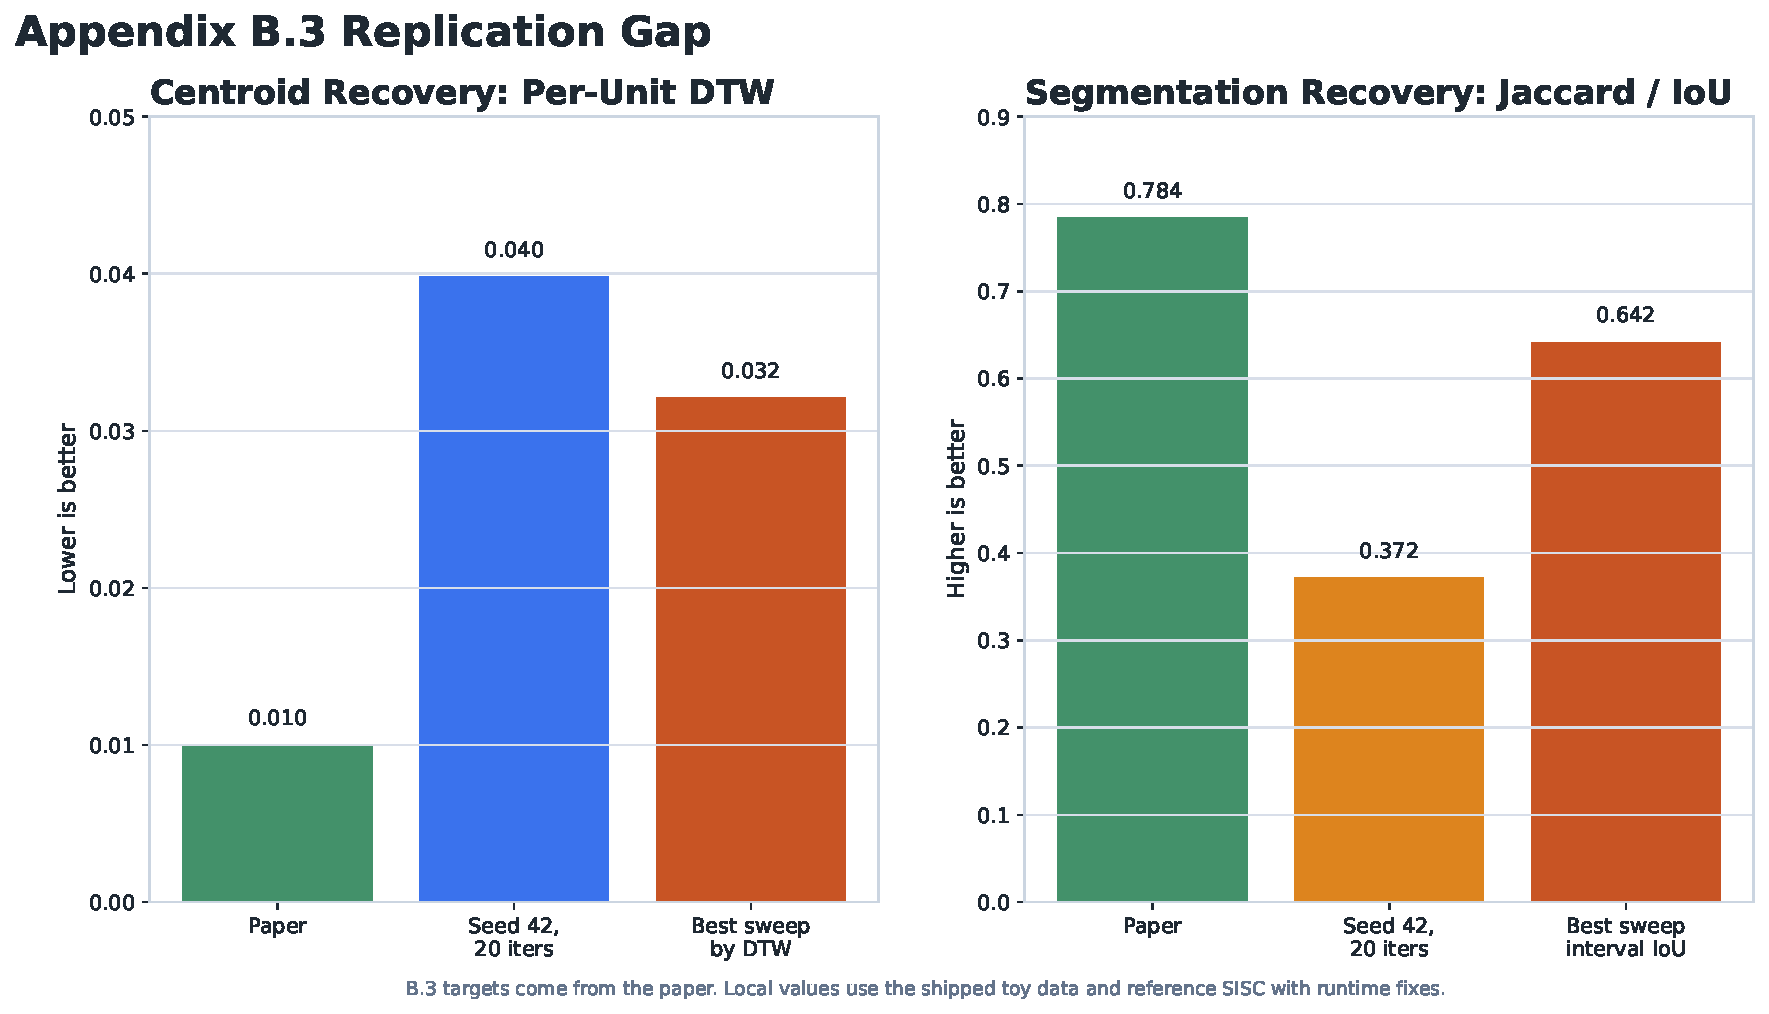
\includegraphics[width=0.92\linewidth]{04_b3_metric_gap.pdf}
  \caption{Appendix B.3 SISC replication gap on the toy data. The best replication runs do not reach the reported centroid or segmentation targets.}
  \label{fig:b3-gap}
\end{figure}

The gap persisted when increasing SISC iterations from 10 to 20 and when changing $l_{\max}$ from 20 to 21. The best centroid metric remained about $3.2\times$ the reported target. This does not invalidate SISC, but exact B.3 reproduction appears to require more detail about the synthetic generator, seed state, one-pattern construction, and metric definitions. We also found portability issues in the downstream setup: the five-year warm-up used for S\&P 500 is not directly portable to shorter GOOG or ZC=F held-out windows, and plotting/downstream helpers can obscure the actual augmentation scale if not audited.

\section{Predictable-drift extension}

\subsection{Diagnostic}

Stylized facts are necessary but not sufficient for finance. A generator can reproduce heavy tails and volatility clustering while encoding a simple conditional mean, such as $r_{t+1} = \rho r_t + \epsilon_{t+1}$. Marginal tests may not detect this, but a trading signal using $r_t$ can.

Motivated by the martingale-difference intuition behind weak-form market efficiency \citep{fama1970efficient}, we fix a small information set
\begin{equation}
  \omega_t =
  \left(1,\ r_t,\ r_{t-1},\ |r_t|,\ |r_{t-1}|\right)^\top
\end{equation}
and a bounded linear class
\begin{equation}
  g_b(\F_t) = b^\top \omega_t, \qquad \norm{b}_2 \leq 1.
\end{equation}
The population predictable-drift violation is
\begin{equation}
  \delta =
  \sup_{\norm{b}_2 \leq 1}
  \left| \E \left[r_{t+1} b^\top \omega_t \right]\right|.
  \label{eq:delta-pop}
\end{equation}
Let $m = \E[r_{t+1}\omega_t]$. By Cauchy-Schwarz, Equation~\ref{eq:delta-pop} has the closed form
\begin{equation}
  \delta = \norm{m}_2.
\end{equation}
The empirical estimator is therefore
\begin{equation}
  \hat{\delta} =
  \left\|
    \frac{1}{T-2}\sum_{t=2}^{T-1} r_{t+1}\omega_t
  \right\|_2.
  \label{eq:delta-hat}
\end{equation}

The statistic decomposes into interpretable components: unconditional drift, first-lag return predictability, second-lag return predictability, and two volatility-conditioned mean terms. In our implementation, returns are standardized using training-split mean and standard deviation only; the constant feature remains equal to one. We compare real data, synthetic data, and a block-shuffled null that preserves the return multiset and some local dependence while disrupting longer chronological alignment.

\subsection{Real-asset calibration}

Before using $\hat{\delta}$ as a rejection statistic, we calibrate it on real held-out assets. For S\&P 500, GOOG, and ZC=F, we start from raw close-price CSVs, use the first $80\%$ of simple returns for standardization, and evaluate the last $20\%$. The null distribution uses 500 replications of 21-day block shuffling on the held-out returns. Table~\ref{tab:real-drift-calibration} shows that all three real held-out paths lie inside their asset-specific 5--95\% null bands, despite retaining heavy tails and volatility clustering. This is a useful sanity check: the diagnostic is not simply rejecting real financial data because it is non-Gaussian.

\begin{table}[h]
  \caption{Real-asset predictable-drift calibration. The null band is the 5--95\% range from 500 block-shuffled held-out paths.}
  \label{tab:real-drift-calibration}
  \centering
  \begin{tabular}{lrrrr}
    \toprule
    Asset & Test obs. & Real $\hat{\delta}$ & Null 5--95\% & ACF$(|r|)$ lag 1 \\
    \midrule
    S\&P 500 & 2018 & 0.0297 & [0.0222, 0.0303] & 0.2165 \\
    GOOG & 755 & 0.0575 & [0.0403, 0.0629] & 0.0935 \\
    ZC=F & 953 & 0.0173 & [0.0150, 0.0259] & 0.1250 \\
    \bottomrule
  \end{tabular}
\end{table}

\subsection{Controlled predictive-alpha test}

We next test whether larger $\hat{\delta}$ corresponds to exploitable predictability. In each of 100 seeds, we simulate a zero-mean heavy-tailed GARCH-like path, keep the evaluation-period magnitude path $|r_t|$ fixed, and replace only the signs. The iid-sign control has no intentional sign predictability; Markov-sign samples have sign persistence $p$. We fit a ridge linear predictor on the first half of each evaluation path using the same feature map $\omega_t$, then evaluate one-step prediction and a sign strategy on the second half.

Table~\ref{tab:drift-alpha} shows the result. The iid-sign and real controls have near-zero out-of-sample correlation, near-50\% directional accuracy, and near-zero strategy Sharpe. At $p=0.85$, the hidden-drift sample has mean $\hat{\delta}=0.5383$, out-of-sample correlation $0.4137$, directional accuracy $79.45\%$, and mean annualized Sharpe $7.68$ with seed standard deviation $1.26$. Across all controlled samples, pooled $\hat{\delta}$ and out-of-sample Sharpe have correlation $0.6414$. Thus the diagnostic is not merely a reporting statistic; it is aligned with artificial alpha.

\begin{table}[t]
  \caption{Controlled predictive-alpha test over 100 seeds. Magnitude paths are fixed within seed; only sign dependence changes.}
  \label{tab:drift-alpha}
  \centering
  \begin{tabular}{lrrrrl}
    \toprule
    Sample & $p$ & $\hat{\delta}$ & OOS corr. & Dir. acc. & Sharpe (sd) \\
    \midrule
    Real evaluation path & -- & 0.1049 & 0.0035 & 0.5021 & 0.10 (0.84) \\
    IID signs & -- & 0.1005 & 0.0017 & 0.5003 & 0.08 (0.69) \\
    Markov signs & 0.65 & 0.2152 & 0.1393 & 0.5909 & 2.15 (1.06) \\
    Markov signs & 0.75 & 0.3717 & 0.2845 & 0.6925 & 4.78 (1.11) \\
    Markov signs & 0.85 & 0.5383 & 0.4137 & 0.7945 & 7.68 (1.26) \\
    Markov signs & 0.90 & 0.6604 & 0.4886 & 0.8526 & 9.65 (1.41) \\
    \bottomrule
  \end{tabular}
\end{table}

The FTS-Diffusion use case is direct: report Equation~\ref{eq:delta-hat} on ordered samples from each rollout protocol, and do not select a protocol only because it improves TATR if its $\hat{\delta}$ lies outside the real/null band. If the statistic is incorporated during training, use it as a validation-selected penalty
\begin{equation}
  \mathcal{L}_{\mathrm{total}}
  =
  \mathcal{L}_{\mathrm{FTS}}
  +
  \lambda \hat{\delta}_{\mathrm{synthetic}}^2.
  \label{eq:drift-penalty}
\end{equation}
The penalty must be computed on ordered return sequences. Applying it across randomly shuffled mini-batches would destroy the time ordering and should only be logged as a proxy, not as the final diagnostic.

\section{Limitations and broader impact}

Our replication is constrained by the information and compute available for this study. Some runs use reference checkpoints rather than a full fresh retraining of all modules. The drift extension is calibrated on real assets and validated in controlled predictive-alpha experiments, but the full FTS-Diffusion drift audit remains to be run on ordered generated samples from every rollout protocol. GOOG and ZC=F have shorter histories than S\&P 500, so the downstream split used for S\&P 500 is not directly portable without changing the question being asked.

The predictable-drift diagnostic is deliberately narrow. It tests a fixed finite-dimensional feature map, not every admissible trading strategy, and it is not a proof of no-arbitrage. Its strength is reproducibility: the statistic is simple, closed-form, and hard to tune after seeing the result.

Synthetic financial data can be beneficial for stress testing, augmentation, and reproducibility, but it can also create misleading evidence if artificial predictability is mistaken for real market structure. Any release of synthetic paths should clearly label them as generated data, document the training period and generation protocol, and avoid implying that downstream forecasting gains translate into tradable performance.

\section{Conclusion}

FTS-Diffusion has the right inductive bias for financial time series: variable-length motifs, pattern-conditioned diffusion, and learned motif evolution. Our replication suggests that the architecture is more robust than the downstream evaluation protocol. Continuous synthetic rollouts can create strong TATR improvements, while independent fixed blocks can fail badly under the same broad data budget. This protocol sensitivity motivates a stricter evaluation standard. Future synthetic-finance benchmarks should report not only stylized facts and forecasting improvements, but also exact rollout protocols and direct predictable-drift diagnostics.

\bibliographystyle{plainnat}
\bibliography{references}

\newpage
\input{checklist.tex}

\end{document}
